\chapter{Arhitektura i dizajn sustava}
		
	Da bi dugoročno uštedjeli vrijeme, uložili smo dio vremena na konfiguriranje CI (continuous integration) i CD (continuous delivery) procesa. Za deploy aplikacije odabrali smo Heroku. Heroku je jedna od najpoznatijih platforma za deployanje aplikacija, a iz šume drugih ističe se svojom jednostavnošću.
	U usporedbi s AWS-ovim servisima koje smo razmatrali, Heroku se sam brine oko instanci i arhitekture sustava na kojem se vrti naša aplikacija.Zbog ograničenih resursa odlučili smo deployati aplikaciju na besplatnu instancu Heroku-a.
	Besplatna instanca Heroku-a ima određena ograničenja, a najupečatljivije od njih je način na koji se pokreće projekt.
	Heroku sam prepoznaje kojeg je tipa projekt pa da deployamo frontend i backend trebamo dvije instance.
	CD je integriran putem gitlab-ovih pipelinesa za koje je bilo potrebno napisati .gitlab-ci.yml datoteku u kojoj smo konfigurirali gitlab-ov pipeline. Gitlab-ov pipeline konfiguriran je tako da se na svaki commit u dev grani izgradi aplikacija, pokrenu i uspješno završe testovi i krene deploy na Heroku.\\
	Da bi osigurali maksimalno vrijeme dostupnosti naše platforme, .yml datoteka također je konfigurirana tako da prilikom commita u master deploya aplikaciju na druge dvije instance.
	Ukupno imamo 4 pokrenute instance Heroku-a, od koje su dvije backend (development i produkcija) ,a dvije frontend (development i produkcija). U skladu s time, aplikacija ima 2 .properties datoteke. Jedna od njih je namijenjena lokalnom izvođenju aplikacije te sadrži postavke lokalne PostgreSQL baze, dok je druga konfigurirana tako da postavke čita iz varijabli okruženja. Varijable okruženja postavljene su na Heroku tako da čak niti pristupom u git repozitorij vanjski korisnik ne može doći do akreditacije (credentials) kojima bi mogao pristupiti bazi.
	
	Prednost ostvarena automatiziranjem deployment procesa jest povećanje vjerojatnosti uspješnosti deploya te povećanje udjela dostupnosti aplikacije zbog dva para instanci servera.
	
	Uvidjevši prednosti korištenja continuous deploymenta, primijenili smo to znanje i na kompajliranje dokumentacije. 
	Unutar repozitorija, osim pipeline-a za deploy, postoji pipeline za automatsko kompajliranje dokumentacije čiji je rezultat .pdf dokument.\\
	
	Potencijalni prostor za napredak bio bi korištenje Docker tehnologije tako da prilikom pokretanja aplikacije korisnik ne mora imati instaliranu PostgreSQL bazu već ju pokrene u Docker kontejneru.\\

	Od mogućih arhitektura sustava, za svoj projekt smo odabrali objektno usmjerenu arhitekturu. Tu arhitekturu smo odabrali zato što se koristi u industriji te je de facto standard razvoja programskih rješenja. Osim toga, ona je fleksibilna, omogućuje recikliranje koda, te logički razdjeljuje sustav na više cjelina, što je bitno s obzirom da više ljudi radi na implementaciji aplikacije. Zahvaljujući modularnosti programskog rješenja, greške su lako ispravljive, a nove mogućnosti dodaju se lako u timu.\\

	Odlučili smo se za web aplikaciju, koja je prilagođena mobilni uređajima, obzirom da glazbenici, a time i bendovi nemaju uvijek pristup računalu, a ne želimo da je korisnik ograničen samo na mobilne uređaje.\\

	Arhitekturu sustava možemo podijeliti na četiri podsustava:
		\begin{itemize}
			\item Web preglednik
			\item Web poslužitelj
    			\item Web aplikacija
			\item Baza podataka
		\end{itemize}


	Korisnik (javnost, glazbenik, bend, administrator) pristupa web aplikaciji uz pomoć svog web preglednika, s time da se u sredini nalazi web poslužitelj. Na njemu se nalazi aplikacija koju on pokreće, te uz pomoć protokola komunicira s korisnicima.\\

	Klijentski (frontend) dio aplikacije omogućuje da korisnik korištenjem sučelja može pristupiti serveru (backend) aplikacije. Ovisno o tome što korisnik hoće, taj server ima mogućnost spajanja na bazu podataka kako bi korisniku prikazao informacije.\\

	Backend je napisan u Javi, a kao razvojni okvir koristimo Java Spring Boot. Dodani su projekti Spring Data kako bi backend mogao lako komunicirati s bazom, Spring Web MVC za rukovanje sa request-ima te Spring Security kako bi zaštitili aplikaciju od vanjskih napada. \\

	\begin{figure}[H]
		\begin{center}
			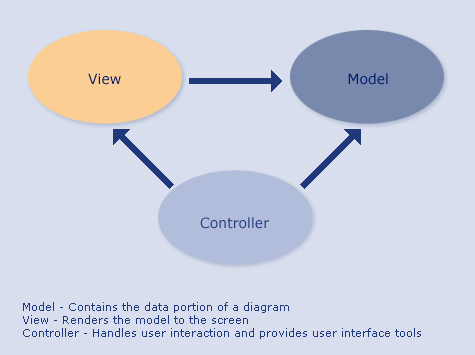
\includegraphics[width=10cm]{slike/mvc.PNG}
		\end{center}
		\caption{Pojednostavljeni prikaz MVC-a}
		\label{fig:mvc}
	\end{figure}

	Za frontend koristimo React. On je moderan i jednostavan framework koji koristi HTML, CSS, JSX i JavaScript uz pomoć kojeg smo napravili sučelje za našu aplikaciju. Uz pomoć React-a možemo lagano komunicirati s backendom koristeći REST.\\




		\section{Baza podataka}
		
		Za potrebe razvoja \textit{Gigera} koristit će se objektno relacijsko mapiranje. To je metoda koja se koristi u objektno-orijentiranim jezicima te se na taj način stvara virtualna objektna baza podataka. Za implementaciju baze podataka odabrali smo PostgreSQL, zbog generalno pozitivnog iskustva u korištenju te implementacije baze podataka u dosadašnjem fakultetskom obrazovanju. Bitno je naglasiti da na osobnim računalima u svrhu razvijanja aplikacije koristimo istu implementaciju baze kao i na web poslužitelju kako bi minimizirali neočekivano ponašanje.
		
		Baza podataka sastoji se od sljedećih entiteta:
		
		\begin{packed_item}
		\item Comment
		\item Message
		\item Conversation
		\item Conversation\_user
		\item System\_person
		\item People
		\item System\_person\_roles
		\item Organizer
		\item Conversation\_band
		\item Band
		\item Gig\_type
		\item Band\_occasions
		\item Occasion
		\item Musician\_occasions
		\item Band\_invited\_back\_up\_members
		\item Band\_invited
		\item Band\_back\_up\_members
		\item Musician\_bands
		\item Post
		\item Musician
		\item Instruments
		\item Instrument
		\item Musician\_gig\_history
		\item Gig
		\item Review\_gig
		\item Review
		
	\end{packed_item}
	
	
	\subsection{Opis tablica}
	
	\textbf{Comment}
	Ovaj entitet sadrži jedan komentar. Sadrži atribute: id komentara,id autora, sadržaj te vrijeme objavljivanja. Ovaj entitet je u \textit{Many-to-One} vezi  sa entitetom: Post i Person.
	\begin{longtabu} to \textwidth {|X[6, l+3]|X[6, l]|X[20, l]|}
		

		\hline \multicolumn{3}{|c|}{\textbf{Comment}}	 \\[3pt] \hline
		\endfirsthead
		
		\hline 
		\endlastfoot
		
		\textbf{id} & BIGINT	&  	jedinstveni identifikator komentara 	\\ \hline
		content & VARCHAR & sadržaj komentara \\ \hline
		posted\_on & TIMESTAMP & datum i vrijeme objave komentara \\ \hline	
		\textit{author\_id} & BIGINT & jedinstveni identifikator autora komentara \\ \hline
		\textit{fk\_post} & BIGINT & jedinstveni identifikator komentara \\ \hline
		
	\end{longtabu}
	
	\textbf{Message}
	Ovaj entitet sadrži informacije o poruci. Sadrži atribute: id poruke, sadržaj poruke, vrijeme kada je poruka poslana, id pošiljatelja i id razgovora. Ovaj entitet je u \textit{Many-to-One} vezi sa entitetom Conversation, Person, Band. Ako je poruka poslana od banda tada mu je fk\_sender null, a ako je poslan od korisnika tada mu je fk\_sender\_band null.
	\begin{longtabu} to \textwidth {|X[6, l+3]|X[6, l]|X[20, l]|}
		
		\hline \multicolumn{3}{|c|}{\textbf{Message}}	 \\[3pt] \hline
		\endfirsthead
		
		\hline
		\endlastfoot
		
		\textbf{id} & BIGINT	&  	jedinstveni identifikator poruke 	\\ \hline
		content	& VARCHAR & sadržaj poruke	\\ \hline
		sent\_time & TIMESTAMP & vrijeme kada je poruka poslana \\ \hline
		\textit{fk\_sender} & BIGINT & jedinstveni identifikator pošiljatelja \\ \hline
		\textit{fk\_sender\_band} & BIGINT & jedinstveni identifikator benda pošiljatelja \\ \hline
		\textit{fk\_converation} & BIGINT & jedinstveni identifikator razgovora \\ \hline
		
	\end{longtabu}
	
	\textbf{Conversation}
	Ovaj entitet sadrži informacije o razgovoru. Sadrži atribute: id razgovora i ime razgovora. Ovaj entitet je u \textit{One-to-Many} vezi  sa entitetima:Message i Person.
	\begin{longtabu} to \textwidth {|X[6, l+3]|X[6, l]|X[20, l]|}
		
		\hline \multicolumn{3}{|c|}{\textbf{Conversation}}	 \\[3pt] \hline
		\endfirsthead
		
		\hline
		\endlastfoot
		
		\textbf{id} & BIGINT	&  	jedinstveni identifikator razgovora 	\\ \hline
		\textit{fk\_band} & BIGINT & jedinstveni identifikator benda \\ \hline
		picture\_url & VARCHAR & url slike razgovora \\ \hline
		title	& VARCHAR &  naziv razgovora	\\ \hline
		
	\end{longtabu}
	
	\textbf{Conversation\_user}
	Ova vezna tablica sadrži informacije o sudjelovanju korisniku u razgovoru. Sadrži atribute: id korisnika i id razgovora.
	\begin{longtabu} to \textwidth {|X[6, l+3]|X[6, l]|X[20, l]|}
		
		\hline \multicolumn{3}{|c|}{\textbf{Conversation\_user}}	 \\[3pt] \hline
		\endfirsthead
		
		\hline
		\endlastfoot
		
		\textbf{fk\_user} & BIGINT	&  	jedinstveni identifikator korisnika	\\ \hline
		\textbf{fk\_conversation}	& BIGINT &  jedinstveni identifikator razgovora	\\ \hline
		
	\end{longtabu}
	
	\textbf {System\_Person}
	Ovaj entitet sadrži podatke korisnika potrebne sustavu za sistemsku logiku.  Sadrži atribute: id korisnika, email, locked i verified zastavice te šifriranu lozinku. Ovaj entitet je u \textit{One-to-One} vezi  sa entitetima:Person, Musician, Organizer.
	\begin{longtabu} to \textwidth {|X[6, l+3]|X[6, l]|X[20, l]|}
		
		\hline \multicolumn{3}{|c|}{\textbf{System\_person}}	 \\[3pt] \hline
		\endfirsthead
		
		\hline
		\endlastfoot
		
		\textbf{id} & BIGINT	&  	jedinstveni identifikator sustavskih podataka o korisniku	\\ \hline
		email & VARCHAR & email adresa osobe \\ \hline
		locked & BOOLEAN & korisnik ima zabranu korištenja aplikacije ili ne \\ \hline
		password\_hash & VARCHAR & hash lozinke osobe \\ \hline
		verified & BOOLEAN & email adresa potvrđena ili ne \\ \hline
		
	\end{longtabu}
	
		\textbf{Person}
	Ovaj entitet sadrži podatke korisnika potrebne za poslovne svrhe.  Sadrži atribute: telefonski broj, url slike korisnika, korisničko ime kojim se predstavlja javnosti. Ovaj entitet je u \textit{One-to-One} vezi  sa entitetima: System\_Person, Musician, Organizer.
	\begin{longtabu} to \textwidth {|X[6, l+3]|X[6, l]|X[20, l]|}
		
		\hline \multicolumn{3}{|c|}{\textbf{Person}}	 \\[3pt] \hline
		\endfirsthead
		
		\hline
		\endlastfoot
		
		\textbf{id} & BIGINT	&  	jedinstveni identifikator korisnika	\\ \hline
		phone\_number & VARCHAR & telefonski broj korisnika \\ \hline
		picture\_url & VARCHAR & url slike korisnika \\ \hline
		username & VARCHAR & korisničko ime korisnika
		
	\end{longtabu}
	
		\textbf{System\_person\_roles}
	Ova tablica sadrži n-torke iz kojih možemo iščitati dodijeljene role pojedinim korisnicima.  Sadrži atribute: system\_person\_id i cjeli broj role koji predstavlja enumeraciju.
	\begin{longtabu} to \textwidth {|X[6, l+3]|X[6, l]|X[20, l]|}
		
		\hline \multicolumn{3}{|c|}{\textbf{System\_person\_roles}}	 \\[3pt] \hline
		\endfirsthead
		
		\hline
		\endlastfoot
		
		\textbf{system\_person\_id} & BIGINT	&  	jedinstveni identifikator sustavskih podataka o korisniku	\\ \hline
		\textbf{roles} & INT & Uloga korisnika \\ \hline
		
		
	\end{longtabu}
	
	\textbf {Organizer}
	Ovaj entitet sadrži informacije o organizatoru. Sadrži atribute: id organizatora te ime organizatora. Ovaj entitet je u \textit{One-to-Many} vezi  sa entitetima: Review\_organizer, Gig te u \textit{One-to-One} vezi sa System\_person, Musician, Person
	\begin{longtabu} to \textwidth {|X[6, l+3]|X[6, l]|X[20, l]|}
		
		\hline \multicolumn{3}{|c|}{\textbf{Organizer}}	 \\[3pt] \hline
		\endfirsthead
		
		\hline
		\endlastfoot
		
		\textbf{id} & BIGINT	&  	jedinstveni identifikator organizatora 	\\ \hline
		manager\_name	& VARCHAR &  ime organizatora	\\ \hline
		
	\end{longtabu}

\textbf{Band}
Ovaj entitet sadrži podatke o kreiranom bendu.  Sadrži atribute: id, opis, datum formiranja, adresu sjedišta, dodatni opis adrese, par koordinata, maksimalnu udaljenost, naziv benda, url slike benda i id voditelja benda. Ovaj entitet je u \textit{Many-to-Many} vezi s Musician za potrebe liste članova te \textit{Many-to-One} vezi s Musician u sklopu voditelja benda 

	\begin{longtabu} to \textwidth {|X[6, l+3]|X[6, l]|X[20, l]|}
		
		\hline \multicolumn{3}{|c|}{\textbf{Band}}	 \\[3pt] \hline
		\endfirsthead
		
		\hline 
		\endlastfoot
		
		\textbf{id} & BIGINT	&  	jedinstveni identifikator benda 	\\ \hline
		bio & VARCHAR & opis benda \\ \hline
		formed\_date & DATE & datum osnutka benda \\ \hline
		address & VARCHAR & adresa benda \\ \hline
		extra\_description & VARCHAR & dodatak opis benda \\ \hline
		x & DOUBLE & x koordinata lokacije \\ \hline
		y & DOUBLE & y koordinata lokacije \\ \hline
		max\_distance & DOUBLE & najveća udaljenost koju bend želi prijeći zbog gaže \\ \hline
		name & VARCHAR & ime benda \\ \hline
		picture\_url & VARCHAR & url slike benda \\ \hline
		\textit{leader\_id}	& BIGINT &  jedinstveni identifikator voditelja benda	\\ \hline 	
		
	\end{longtabu}
	
			\textbf {Gig\_type}
	Ovo je vezna tablica iz koje se mogu iščitati koje sve vrste nastupa izvodi određen bend.  Sadrži atribute: band\_id i naziv tipa nastupa.
	\begin{longtabu} to \textwidth {|X[6, l+3]|X[6, l]|X[20, l]|}

		\hline \multicolumn{3}{|c|}{\textbf{Gig\_type}}	 \\[3pt] \hline
		\endfirsthead

		\hline
		\endlastfoot

		\textbf{band\_id} &  BIGINT	&  	jedinstveni identifikator benda 	\\ \hline
		\textbf{gig\_type}	& VARCHAR &  vrsta nastupa	\\ \hline

	\end{longtabu}

				\textbf {Band\_occasions}
	Ovo je vezna tablica iz koje se mogu iščitati zauzeti termini za pojedini band.  Sadrži atribute: identifikator benda i identifikator termina.
	\begin{longtabu} to \textwidth {|X[6, l+3]|X[6, l]|X[20, l]|}

		\hline \multicolumn{3}{|c|}{\textbf{Band\_occasions}}	 \\[3pt] \hline
		\endfirsthead

		\hline
		\endlastfoot

		\textbf{occasion\_id} &  BIGINT	&  	jedinstveni identifikator događaja 	\\ \hline
		\textbf{band\_id} &  BIGINT	&  	jedinstveni identifikator benda koji sudjeluje na događaju 	\\ \hline

	\end{longtabu}


		\textbf{Occasion}
	Ovaj entitet sadrži podatke o nekom terminu.  Sadrži atribute: id termina, opis, datum, zastavicu privatnosti. Ovaj entitet je u \emph{Many-to-One} vezi  sa entitetima: Musician, Band.
	\begin{longtabu} to \textwidth {|X[6, l+3]|X[6, l]|X[20, l]|}
		
		\hline \multicolumn{3}{|c|}{\textbf{Occasion}}	 \\[3pt] \hline
		\endfirsthead
		
		\hline 
		\endlastfoot
		
		\textbf{id} &  BIGINT	&  	jedinstveni identifikator događaja 	\\ \hline
		description & VARCHAR & opis događaja \\ \hline
		local\_date & DATE & datum održavanja događaja \\ \hline
		personal\_occasion & BOOLEAN & privatan događaj ili ne \\ \hline

		
		
	\end{longtabu}
	
		\textbf{Musician\_occasions}
	Ovo je vezna tablica iz koje se mogu iščitati zauzeti termini za pojedinog glazbenika.  Sadrži atribute: identifikator glazbenika i identifikator termina.
	\begin{longtabu} to \textwidth {|X[6, l+3]|X[6, l]|X[20, l]|}
		
		\hline \multicolumn{3}{|c|}{\textbf{Musician\_occasions}}	 \\[3pt] \hline
		\endfirsthead
		
		\hline 
		\endlastfoot
		
		\textbf{musician\_id} &  BIGINT	&  	jedinstveni identifikator glazbenika 	\\ \hline
		\textbf{occasions\_id} &  BIGINT	&  	jedinstveni identifikator termina	\\ \hline
		
		
	\end{longtabu}
	
		\textbf{Band\_invited\_back\_up\_members}
	Ovo je vezna tablica iz koje se mogu iščitati poslane i ne odgovorene pozivnice za pričuvnog člana benda.  Sadrži atribute: identifikator glazbenika i identifikator benda.
	\begin{longtabu} to \textwidth {|X[6, l+11]|X[6, l]|X[20, l]|}
		
		\hline \multicolumn{3}{|c|}{\textbf{Band\_invited\_back\_up\_members}}	 \\[3pt] \hline
		\endfirsthead
		
		\hline 
		\endlastfoot
		
		\textbf{band\_id} &  BIGINT	&  	jedinstveni identifikator benda 	\\ \hline
		\textbf{invited\_back\_up\_members\_id} &  BIGINT	&  	jedinstveni identifikator glazbenika pozvanih u bend kao rezerva	\\ \hline
		
		
	\end{longtabu}
	
		\textbf{Band\_invited}
	Ovo je vezna tablica iz koje se mogu iščitati poslane i ne odgovorene pozivnice za člana benda.  Sadrži atribute: identifikator glazbenika i identifikator benda. . Ovaj entitet je u \textit{Many-to-One} vezi s entitetima: Band i Musician.
	\begin{longtabu} to \textwidth {|X[6, l+3]|X[6, l]|X[20, l]|}
		
		\hline \multicolumn{3}{|c|}{\textbf{Band\_invited}}	 \\[3pt] \hline
		\endfirsthead
		
		\hline 
		\endlastfoot
		
		\textbf{band\_id} &  BIGINT	&  	jedinstveni identifikator benda 	\\ \hline
		\textbf{invited\_id} &  BIGINT	&  	jedinstveni identifikator glazbenika pozvanih u bend	\\ \hline
		
		
	\end{longtabu}
	
			\textbf {Band\_back\_up\_members}
	Ovo je vezna tablica iz koje se mogu iščitati rezervni članovi bendova.  Sadrži atribute: identifikator glazbenika i identifikator benda.
	\begin{longtabu} to \textwidth {|X[6, l+10]|X[6, l]|X[20, l]|}
		
		\hline \multicolumn{3}{|c|}{\textbf{Band\_back\_up\_members}}	 \\[3pt] \hline
		\endfirsthead
		
		\hline 
		\endlastfoot
		
		\textbf{band\_id} &  BIGINT	&  	jedinstveni identifikator benda 	\\ \hline
		\textbf{invited\_back\_up\_members\_id} &  BIGINT	&  	jedinstveni identifikator glazbenika koji su rezervni članovi	\\ \hline
		
		
	\end{longtabu}
	
			\textbf {Musician\_bands}
	Ovo je vezna tablica iz koje se mogu iščitati članovi bendova.  Sadrži atribute: identifikator glazbenika i identifikator benda.Ovaj entitet je u \emph{Many-to-One} vezi s entitetima: Band i Musician.
	\begin{longtabu} to \textwidth {|X[6, l+3]|X[6, l]|X[20, l]|}
		
		\hline \multicolumn{3}{|c|}{\textbf{Musician\_bands}}	 \\[3pt] \hline
		\endfirsthead
		
		\hline 
		\endlastfoot
		
		\textbf{fk\_musician} & BIGINT	&  	jedinstveni identifikator glazbenika 	\\ \hline
		\textbf{fk\_band}	& BIGINT &  jedinstveni identifikator benda	\\ \hline
		
	\end{longtabu}
	
	\textbf{Post}
	Ovaj entitet sadrži podatke o objavi.  Sadrži atribute: id objave, sadržaj, datum i vrijeme objave, identifikator korisnika ili banda (autora). Ovaj entitet je u \textit{One-to-Many} vezi  sa entitetima: comment, u \emph{Many-to-one} sa entitetima: Person, Band.
	\begin{longtabu} to \textwidth {|X[6, l+3]|X[6, l]|X[20, l]|}
		
		\hline \multicolumn{3}{|c|}{\textbf{Post}}	 \\[3pt] \hline
		\endfirsthead
		
		\hline 
		\endlastfoot
		
		\textbf{id} & BIGINT	&  	jedinstveni identifikator objave 	\\ \hline
		content & VARCHAR & sadržaj objave \\ \hline
		published\_on & TIMESTAMP & datum i vrijeme objave \\ \hline
		\textit{fk\_band} & BIGINT & jedinstveni identifikator benda \\ \hline
		\textit{fk\_user} & BIGINT & jedinstveni identifikator korisnika koji je napisao objavu \\ \hline
		
	\end{longtabu}
	
		\textbf {Musician}
	Ovaj entitet sadrži informacije o glazbeniku. Sadrži atribute: id glazbenika, oznaku za privatan kalendar te opis glazbenika. Ovaj entitet je u \textit{One-to-Many} vezi s entitetima: Musician\_gig\_history, Band\_invited\_back\_up\_members, Instruments, Post, Band\_invited, Band\_back\_up\_members, Musician\_ocassions, Band i People.
	\begin{longtabu} to \textwidth {|X[6, l+3]|X[6, l]|X[20, l]|}
		
		\hline \multicolumn{3}{|c|}{\textbf{Musician}}	 \\[3pt] \hline
		\endfirsthead
		
		\hline 
		\endlastfoot
		
		\textbf{id} & BIGINT	&  	jedinstveni identifikator glazbenika 	\\ \hline	
		bio	& VARCHAR &  opis glazbenika	\\ \hline 
		public\_calendar & BOOLEAN & kalendar glazbenika javan ili ne \\ \hline
			
		
	\end{longtabu}
	
	\textbf{Instruments}
	Ovaj entitet sadrži informacije o instrumentima koje sviraju glazbenici. Sadrži atribute: id instrumenta te id glazbenika. Ovaj entitet je u \textit{Many-to-One} vezi s entitetima: Musician te Instrument.
	\begin{longtabu} to \textwidth {|X[6, l+3]|X[6, l]|X[20, l]|}
		
		\hline \multicolumn{3}{|c|}{\textbf{Instruments}}	 \\[3pt] \hline
		\endfirsthead
		
		\hline 
		\endlastfoot
		
		\textbf{instruments\_id} & BIGINT & jedinstveni identifikator instrumenta \\ \hline
		\textbf{musician} & BIGINT	&  	jedinstveni identifikator glazbenika	\\ \hline
		
		
	\end{longtabu}
	
	\textbf{Instrument}
	Ovaj entitet sadrži informacije o instrumentima. Sadrži atribute: id instrumenta, ime instrumenta te vrstu instrumenta. Ovaj entitet je u \emph{One-to-Many} vezi s entitetom Instrument.
	\begin{longtabu} to \textwidth {|X[6, l+3]|X[6, l]|X[20, l]|}
		
		\hline \multicolumn{3}{|c|}{\textbf{Instrument}}	 \\[3pt] \hline
		\endfirsthead
		
		\hline 
		\endlastfoot
		
		\textbf{id} & BIGINT & jedinstveni identifikator instrumenta \\ \hline
		name & VARCHAR & ime instrumenta \\ \hline
		type & INT & vrsta instrumenta \\ \hline
		
		
	\end{longtabu}
	
		\textbf{Musician\_gig\_history}
	Ovo je vezna tablica iz koje se može iščitati povijest nastupa glazbenika.  Sadrži atribute: identifikator glazbenika i identifikator nastupa.
	\begin{longtabu} to \textwidth {|X[6, l+3]|X[6, l]|X[20, l]|}
		
		\hline \multicolumn{3}{|c|}{\textbf{Musician\_gig\_history}}	 \\[3pt] \hline
		\endfirsthead
		
		\hline 
		\endlastfoot
		
		\textbf{fk\_musician} & BIGINT & jedinstveni identifikator glazbenika \\ \hline
		\textbf{fk\_gig} & BIGINT & jedinstveni identifikator nastupa \\ \hline
		
		
		
	\end{longtabu}
	
	\textbf {Gig}
	Ovaj entitet sadrži informacije o nastupima. Sadrži atribute: id nastupa, datum i vrijeme održavanja nastupa, opis nastupa, očekivano trajanje nastupa, oznaku za postignut dogovor, vrsta nastupa, adresa održavanja nastupa, dodatan opis nastupa, x koordinata lokacije, y koordinata lokacije, oznaku za privatan nastup, preporučenu cijenu ulaznice, id organizatora te id benda. Ovaj entitet je u \textit{Many-to-One} vezi s entitetom Organizer te \textit{One-to-Many} vezi s entitetima: Musician\_gig\_history, Review\_gig i Band.
	\begin{longtabu} to \textwidth {|X[6, l+3]|X[6, l]|X[20, l]|}
		
		\hline \multicolumn{3}{|c|}{\textbf{Gig}}	 \\[3pt] \hline
		\endfirsthead
		
		\hline 
		\endlastfoot
		
		\textbf{id} & BIGINT	&  	jedinstveni identifikator nastupa 	\\ \hline
		date\_time & TIMESTAMP & datum i vrijeme održavanja nastupa \\ \hline
		description & VARCHAR & opis nastupa \\ \hline
		expected\_duration & VARCHAR & očekivano trajanje nastupa \\ \hline
		final\_deal\_achieved & BOOLEAN & dogovor postignut ili ne \\ \hline
		gig\_type & INT & vrsta nastupa \\ \hline
		address & VARCHAR & adresa održavanja nastupa \\ \hline
		extra\_description & VARCHAR & dodatan opis nastupa \\ \hline
		x & DOUBLE & x koordinata lokacije \\ \hline
		y & DOUBLE & y koordinata lokacije \\ \hline
		private\_gig & BOOLEAN & nastupa privatan ili ne \\ \hline
		proposed\_price & INT & preporučena cijena ulaznice \\ \hline
		\textit{organizer\_id}	& BIGINT &  jedinstveni identifikator organizatora	\\ \hline 	
		\textit{band\_id}	& BIGINT &  jedinstveni identifikator benda	\\ \hline 	
		
	\end{longtabu}
	
	\textbf {Review\_gig}
	Ovaj entitet sadrži informacije za recenziju nastupa. Sadrži atribute: id nastupa i id recenzije. Ovaj entitet je u \textit{Many-to-One} vezi  sa entitetima:Gig i Review.
	\begin{longtabu} to \textwidth {|X[6, l+3]|X[6, l]|X[20, l]|}
		
		\hline \multicolumn{3}{|c|}{\textbf{Review\_gig}}	 \\[3pt] \hline
		\endfirsthead
		
		\hline 
		\endlastfoot
		
		\textbf{fk\_gig} & BIGINT	&  	jedinstveni identifikator nastupa 	\\ \hline
		\textbf{fk\_review}	& BIGINT &  jedinstveni identifikator recenzije	\\ \hline 		
		
	\end{longtabu}
	
	\textbf{Review}
	\textit{Ovaj entitet sadrži informacije za recenziju. Sadrži atribute: id recenzije, sadržaj recenzije benda, sadržaj recenzije organizatora, vrijeme objave recenzije, ocjenu benda, ocjenu organizatora te id autora. Ovaj entitet je u \textit{One-to-Many} vezi  sa entitetima: Review\_band, Review\_gig, Review\_organizer i Review\_musician.}
	
	\begin{longtabu} to \textwidth {|X[6, l+14]|X[6, l+2]|X[20, l]|}
		
		\hline \multicolumn{3}{|c|}{\textbf{Review}}	 \\[3pt] \hline
		\endfirsthead
		
		\hline
		\endlastfoot
		
		\textbf{id} & BIGINT	&  	jedinstveni identifikator recenzije 	\\ \hline
		content\_of\_review\_for\_band	& VARCHAR &  sadržaj komentara benda	\\ \hline
		content\_of\_review\_for\_organizer	& VARCHAR &  sadržaj komentara organizatora	\\ \hline
		created & TIMESTAMP & vrijeme objave komentara \\ \hline
		grade\_band & INT & ocjena benda \\ \hline
		grade\_organizer & INT & ocjena organizatora  \\ \hline
		\textit{author\_id} & BIGINT	& jedinstveni identifikator korisnika koji je autor recenzije	\\ \hline
		
		
	\end{longtabu}
	

		
	

			
			\subsection{Dijagram baze podataka}
			
			\begin{figure}[H]
			\begin{center}
				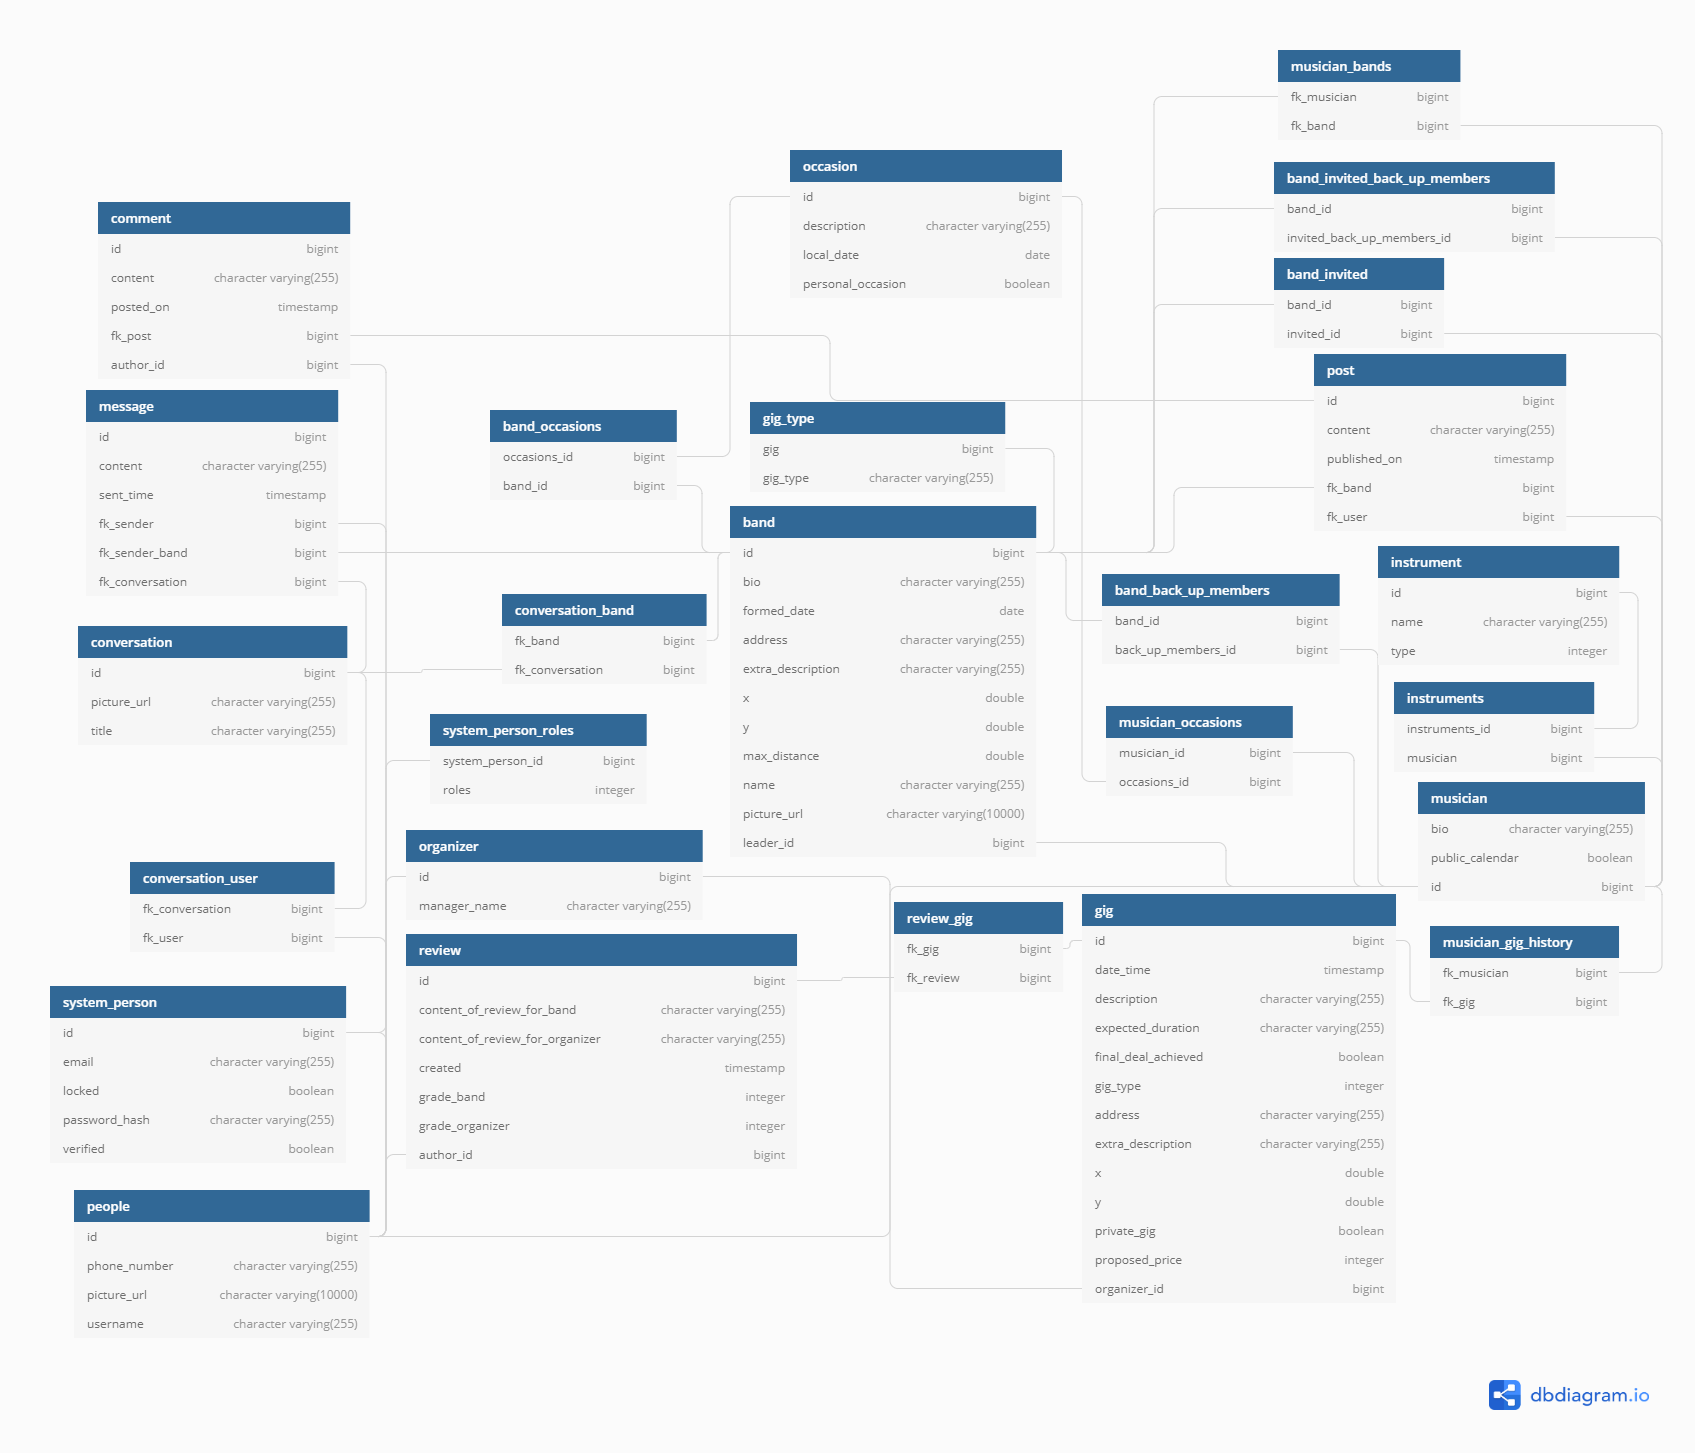
\includegraphics[width=17cm]{slike/ERModel.PNG}
			\end{center}
			\caption{Dijagram baze podataka}
			\label{fig:dijagramBaze}
		\end{figure}
			
			
			
		\section{Dijagram razreda}
		
			\textit{Potrebno je priložiti dijagram razreda s pripadajućim opisom. Zbog preglednosti je moguće dijagram razlomiti na više njih, ali moraju biti grupirani prema sličnim razinama apstrakcije i srodnim funkcionalnostima.}\\
			
			\textbf{\textit{dio 1. revizije}}\\
			
			\textit{Prilikom prve predaje projekta, potrebno je priložiti potpuno razrađen dijagram razreda vezan uz \textbf{generičku funkcionalnost} sustava. Ostale funkcionalnosti trebaju biti idejno razrađene u dijagramu sa sljedećim komponentama: nazivi razreda, nazivi metoda i vrste pristupa metodama (npr. javni, zaštićeni), nazivi atributa razreda, veze i odnosi između razreda.}\\
			
			\textbf{\textit{dio 2. revizije}}\\			
			
			\textit{Prilikom druge predaje projekta dijagram razreda i opisi moraju odgovarati stvarnom stanju implementacije}
			
			... 
			
			
			Na slici 4.3 prikazan je Controllers dio backend aplikacije. Controlleri su jedina izložena točka u aplikaciji te nad njima frontend izvršava upite. Svi Controller-i su zaštićeni Spring Security-jem te se prije svakog propuštanja zahtjeva na Controller autorizira token koji se nalazi u zaglavlju zahtjeva. Jedina iznimka su Controller-i koji služe za registraciju i prijavu. Nakon što se zahtjev autorizira Controller-i pozivaju servisni sloj aplikacije te od njih zahtjevaju da izvrše dio poslovne logike za koju su napisani. Povratni tip Controller-a su DTO-ovi (Data Transfer Objects) prikazani na slici 4.4. Njima se na frontend vraća samo dio informacije prikupljene od servisa.  
			
			\eject
			
			\begin{figure}[H]
				\begin{center}
					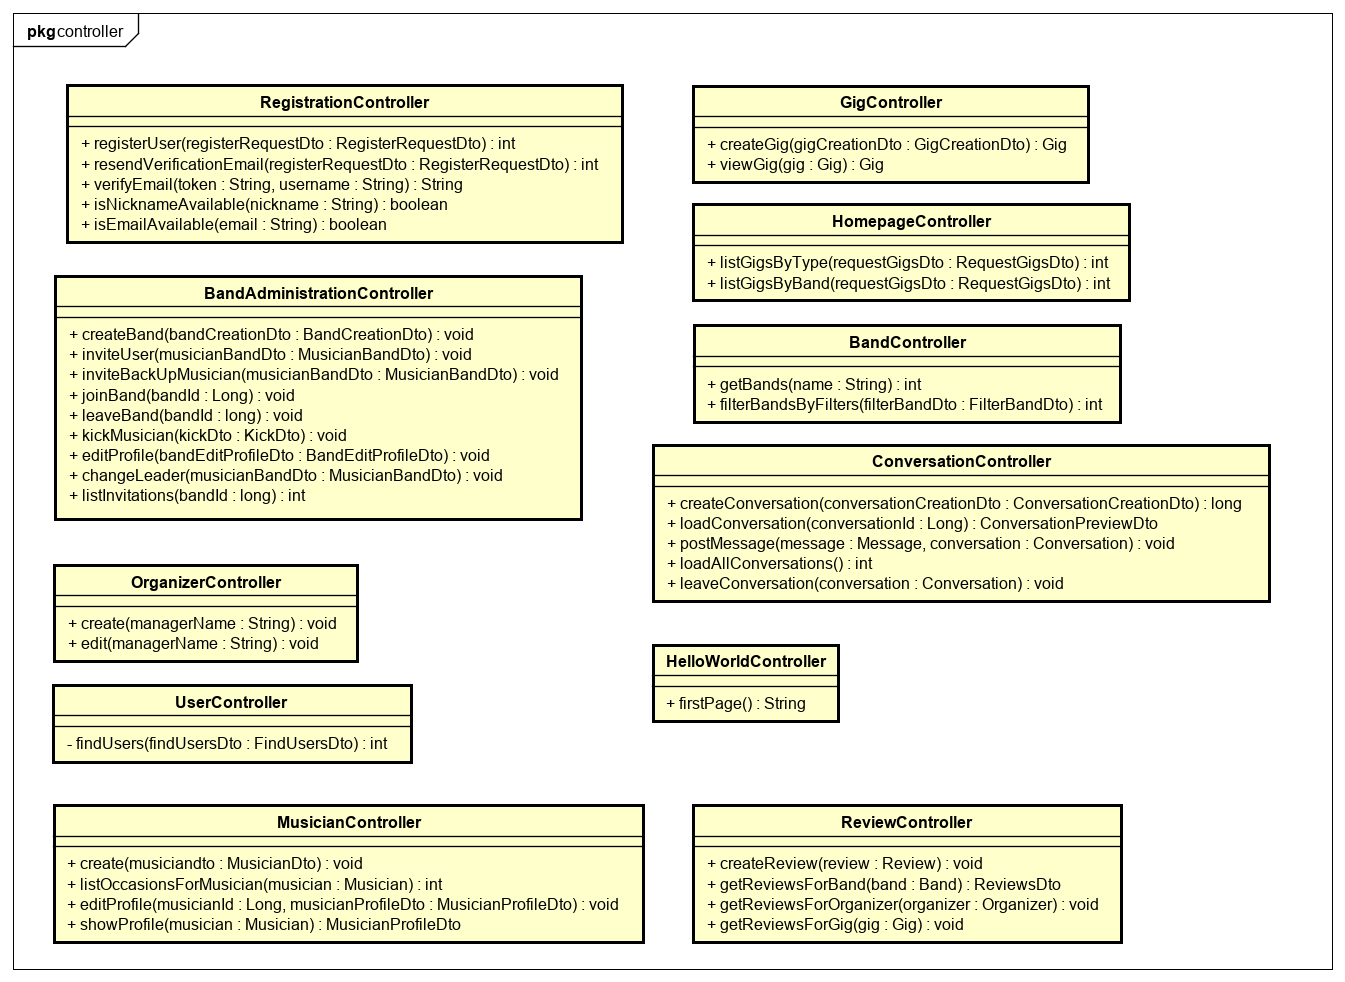
\includegraphics[width=17cm]{slike/kontroleri.PNG}
				\end{center}
				\caption{Dijagram razreda - dio Controllers}
				\label{fig:kontroleri}
			\end{figure}
		
			Slika 4.4 prikazuje DTO-ove kojima backend dio aplikacije komunicira s frontendom. DTO-ove smo modelirali tako da izbjegnemo kružne reference objekata koje dobijemo iz baze podataka. Kao posljedica, DTO-ovi sadrže uglavnom primitivne tipove ili neke druge DTO-ove (npr. ConversationPreviewDTO sadrži listu PersonPreviewDTO koji predstavljaju sudionike razgovora). DTO-ove koristimo u oba smjera komunikacije backenda i frontenda.
			
			
			\begin{figure}[H]
				\begin{center}
					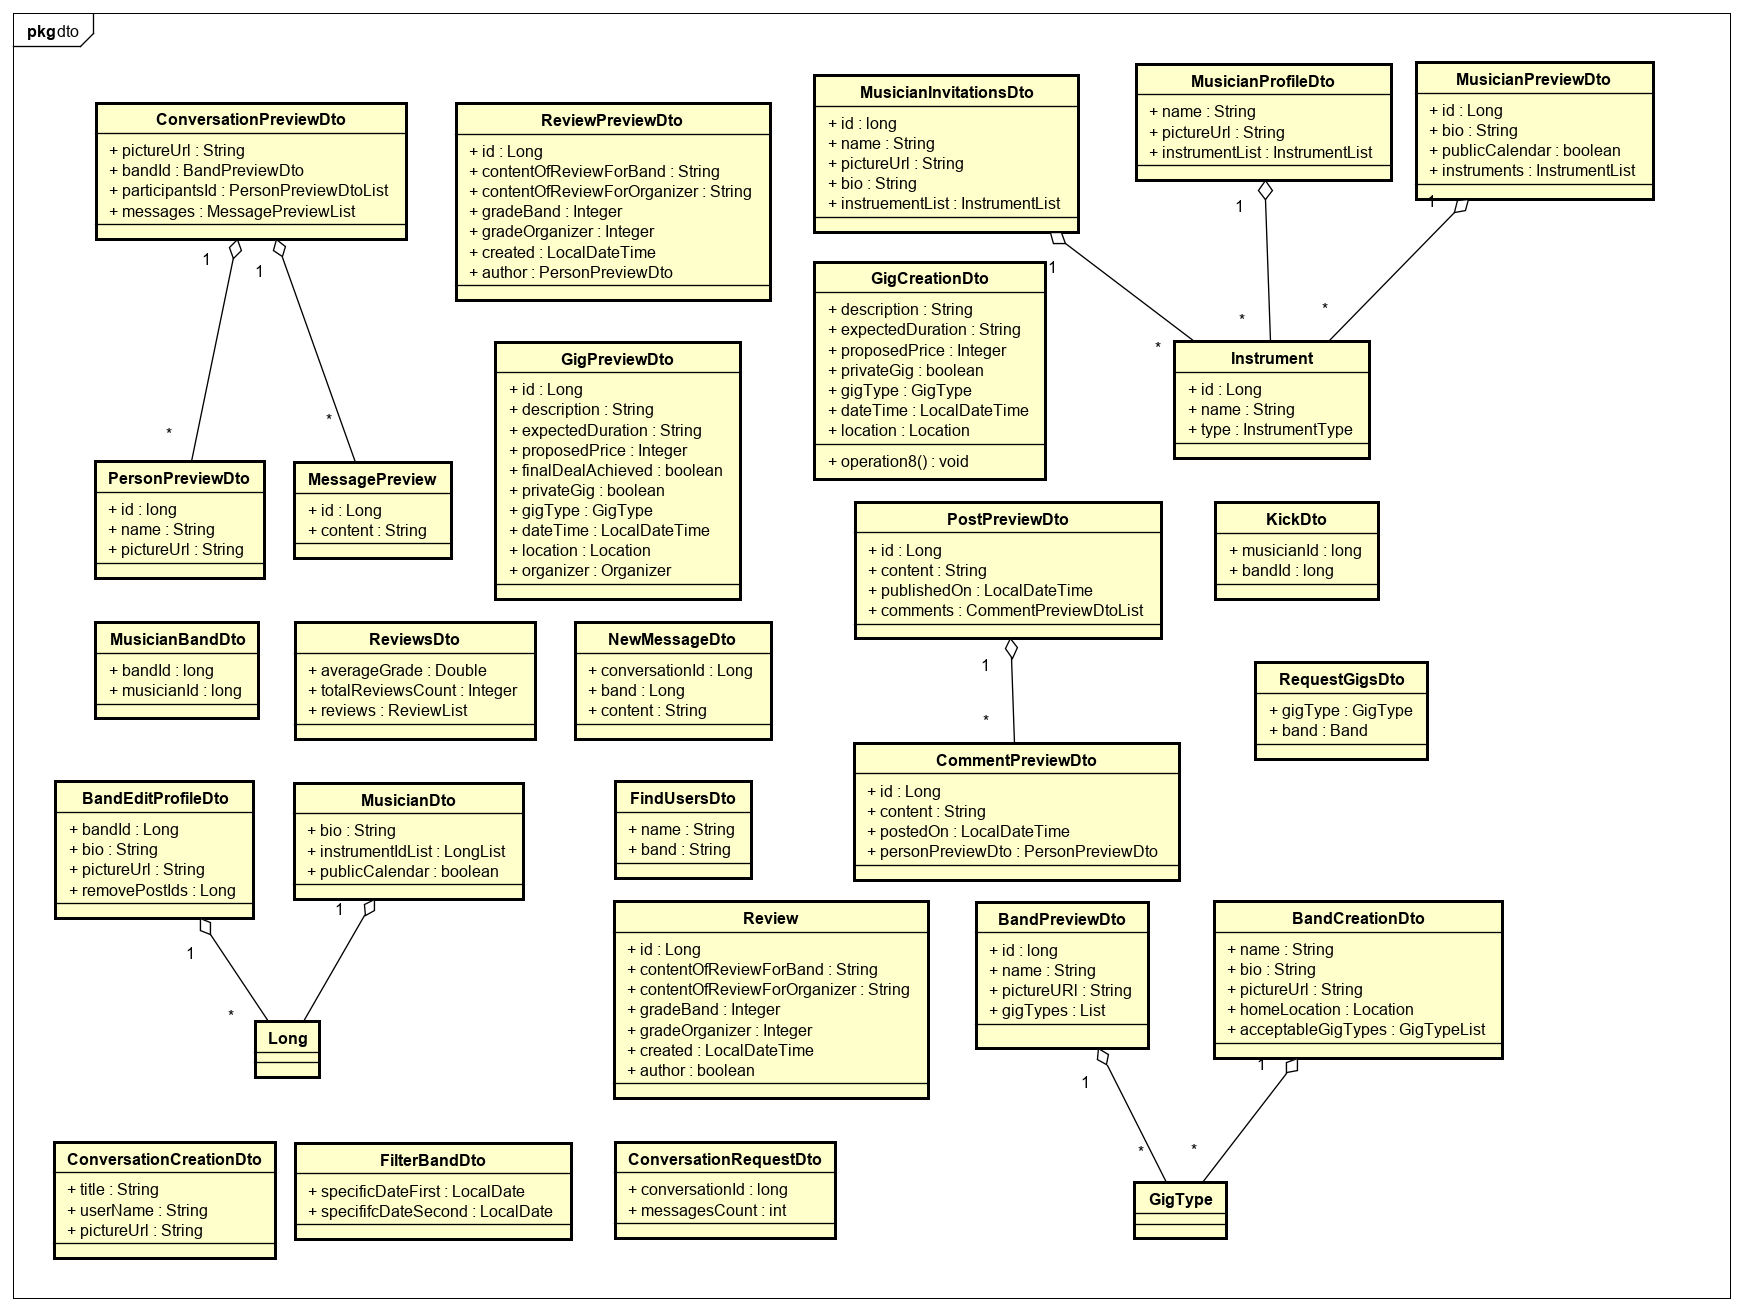
\includegraphics[width=17cm]{slike/DTO.PNG}
				\end{center}
				\caption{Dijagram razreda - dio Data transfer objects}
				\label{fig:dto}
			\end{figure}
		
		Slika 4.5 prikazuje dijagram razreda servisnog sloja. Servisi komuniciraju s repozitorijima koji pristupaju bazi i Controller-ima od kojih dobivaju i kojima vraćaju podatke. Servisi iz baze dobivaju instance objekata koji mogu biti povezani s drugim podatcima, itd. i njihov je cilj poštivajući poslovnu logiku obraditi te podatke i kao rezultat svog izvođenja vraćaju DTO-ove. Servisi sadrže svu poslovnu logiku. Gotovo svaki Controller ima pripadajući servis, a svaki je servis logički objedinjen skup funkcija poslovne logike. Iznimke koje se bacaju u servisima omataju se GigerException-om koji nasljeđuje RuntimeException. Ako se pogreška propagira iz sustava, možemo provjeriti njezin tip te ako je zamotana u GigerException, znači da je to iznimka koju smo očekivali, u protivnom je došlo do neočekivane situacije u sustavu.
		
		\begin{figure}[H]
			\begin{center}
				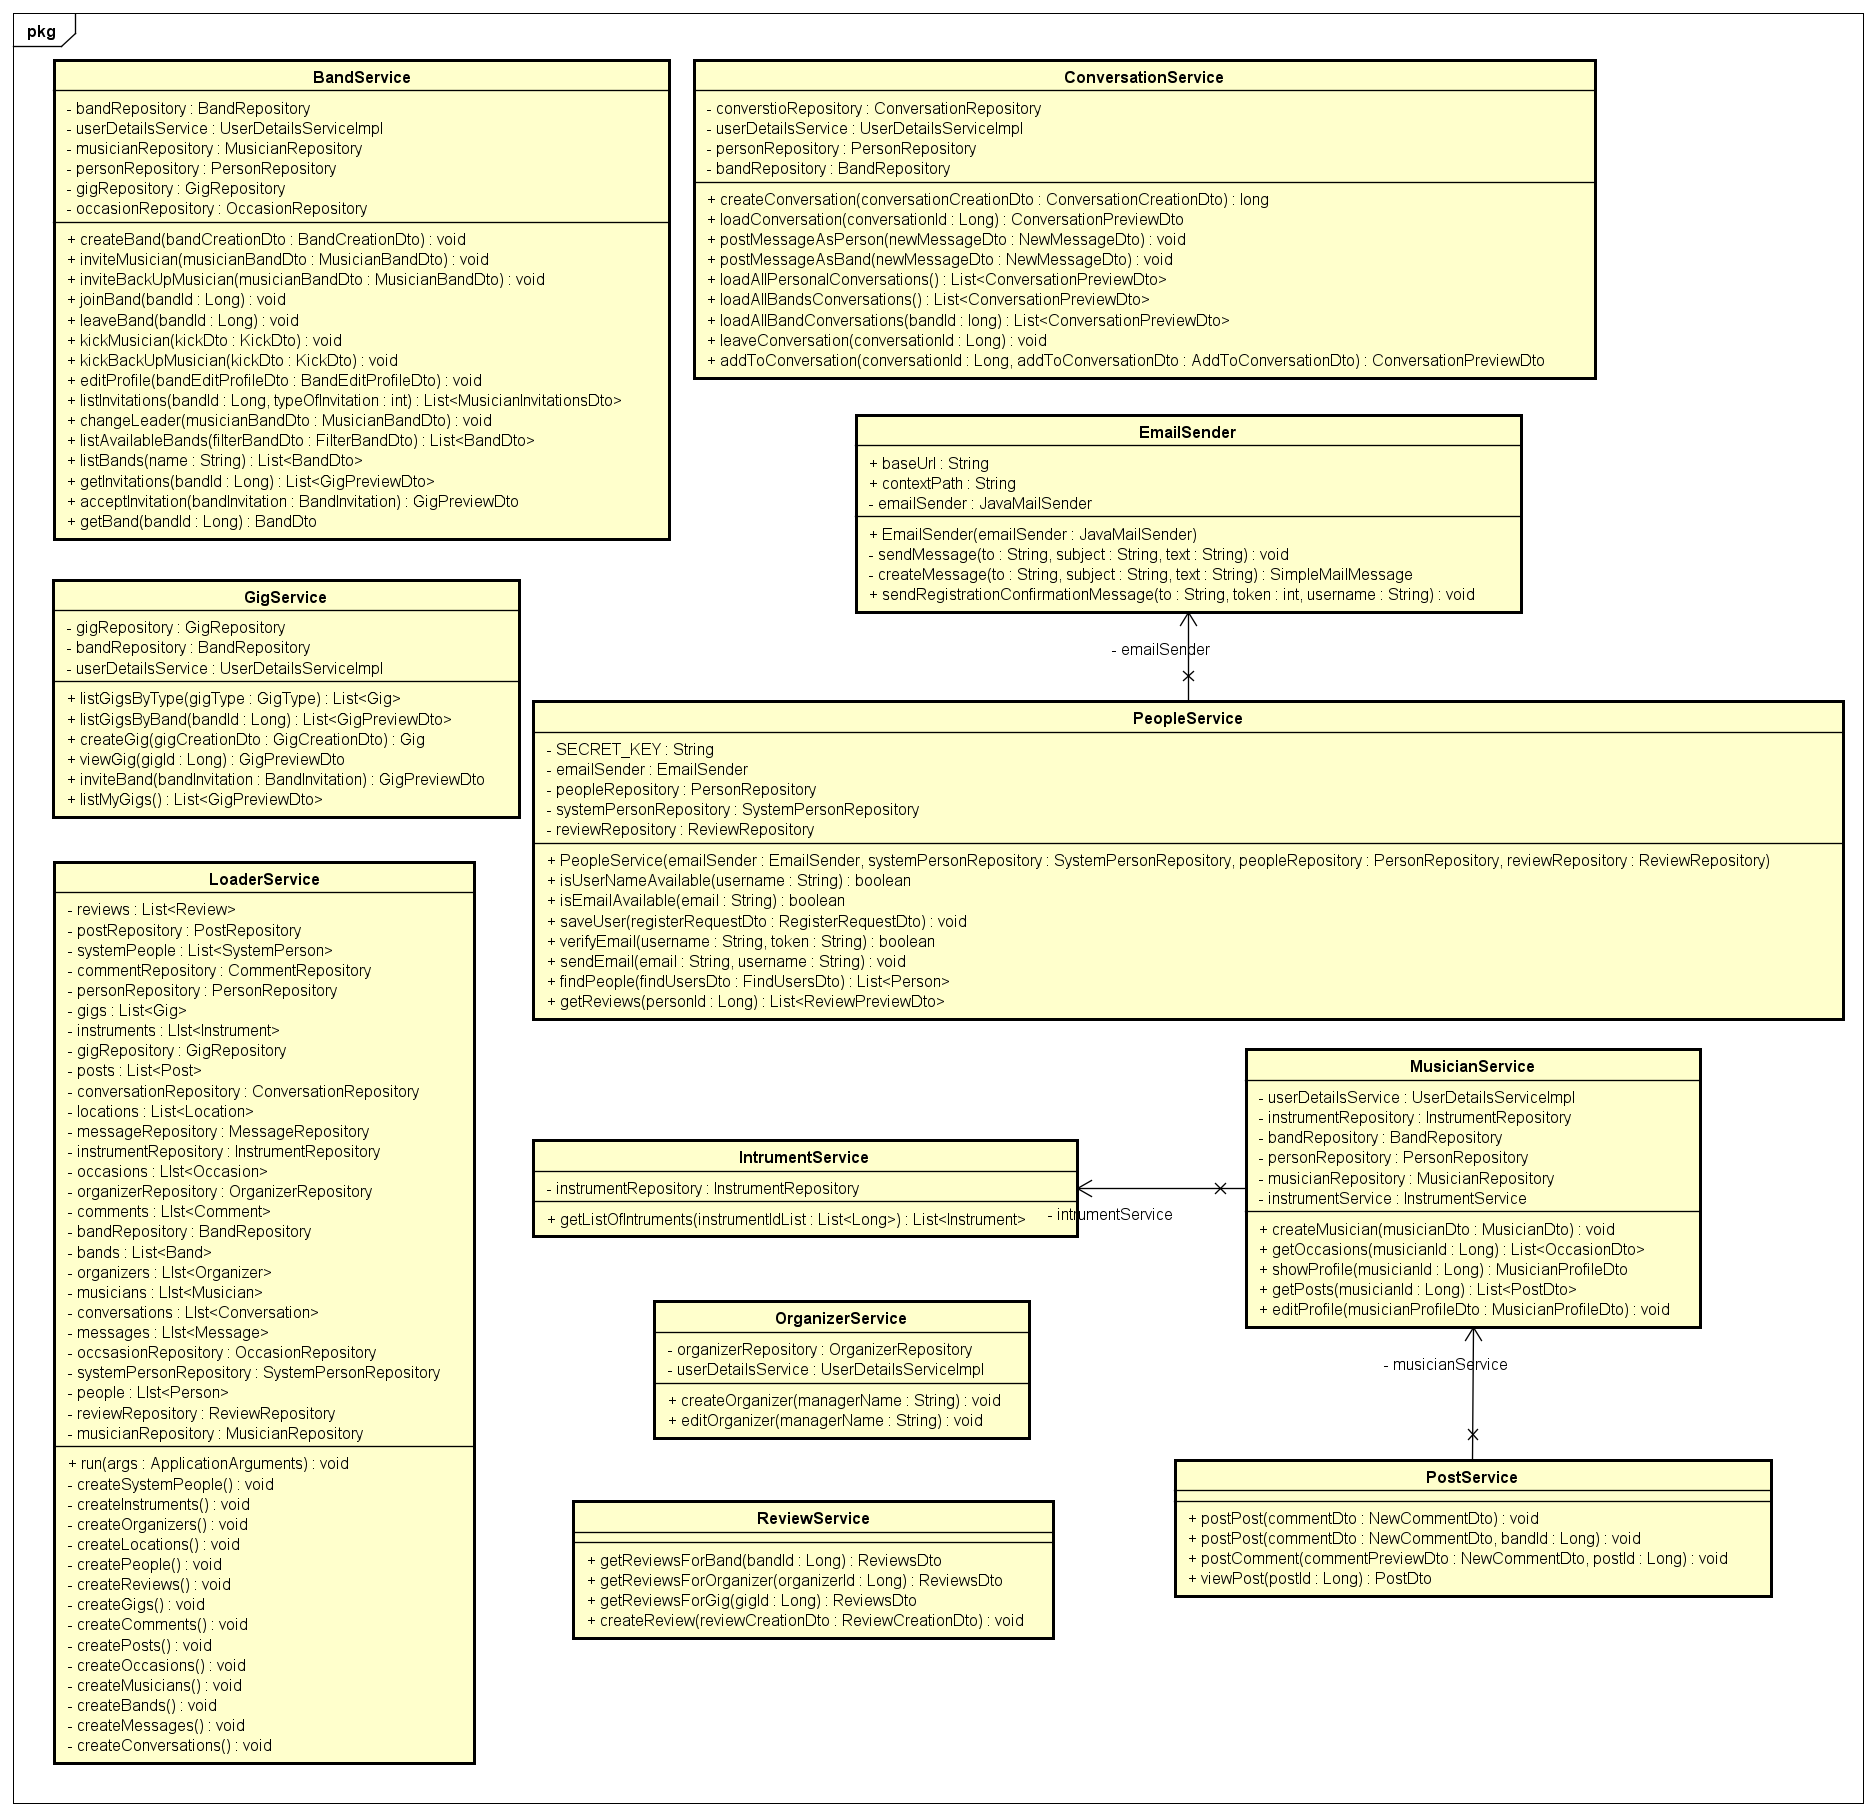
\includegraphics[width=17cm]{slike/service.PNG}
			\end{center}
			\caption{Dijagram razreda - dio Service}
			\label{fig:service}
		\end{figure}
	
		\begin{figure}[H]
			\begin{center}
				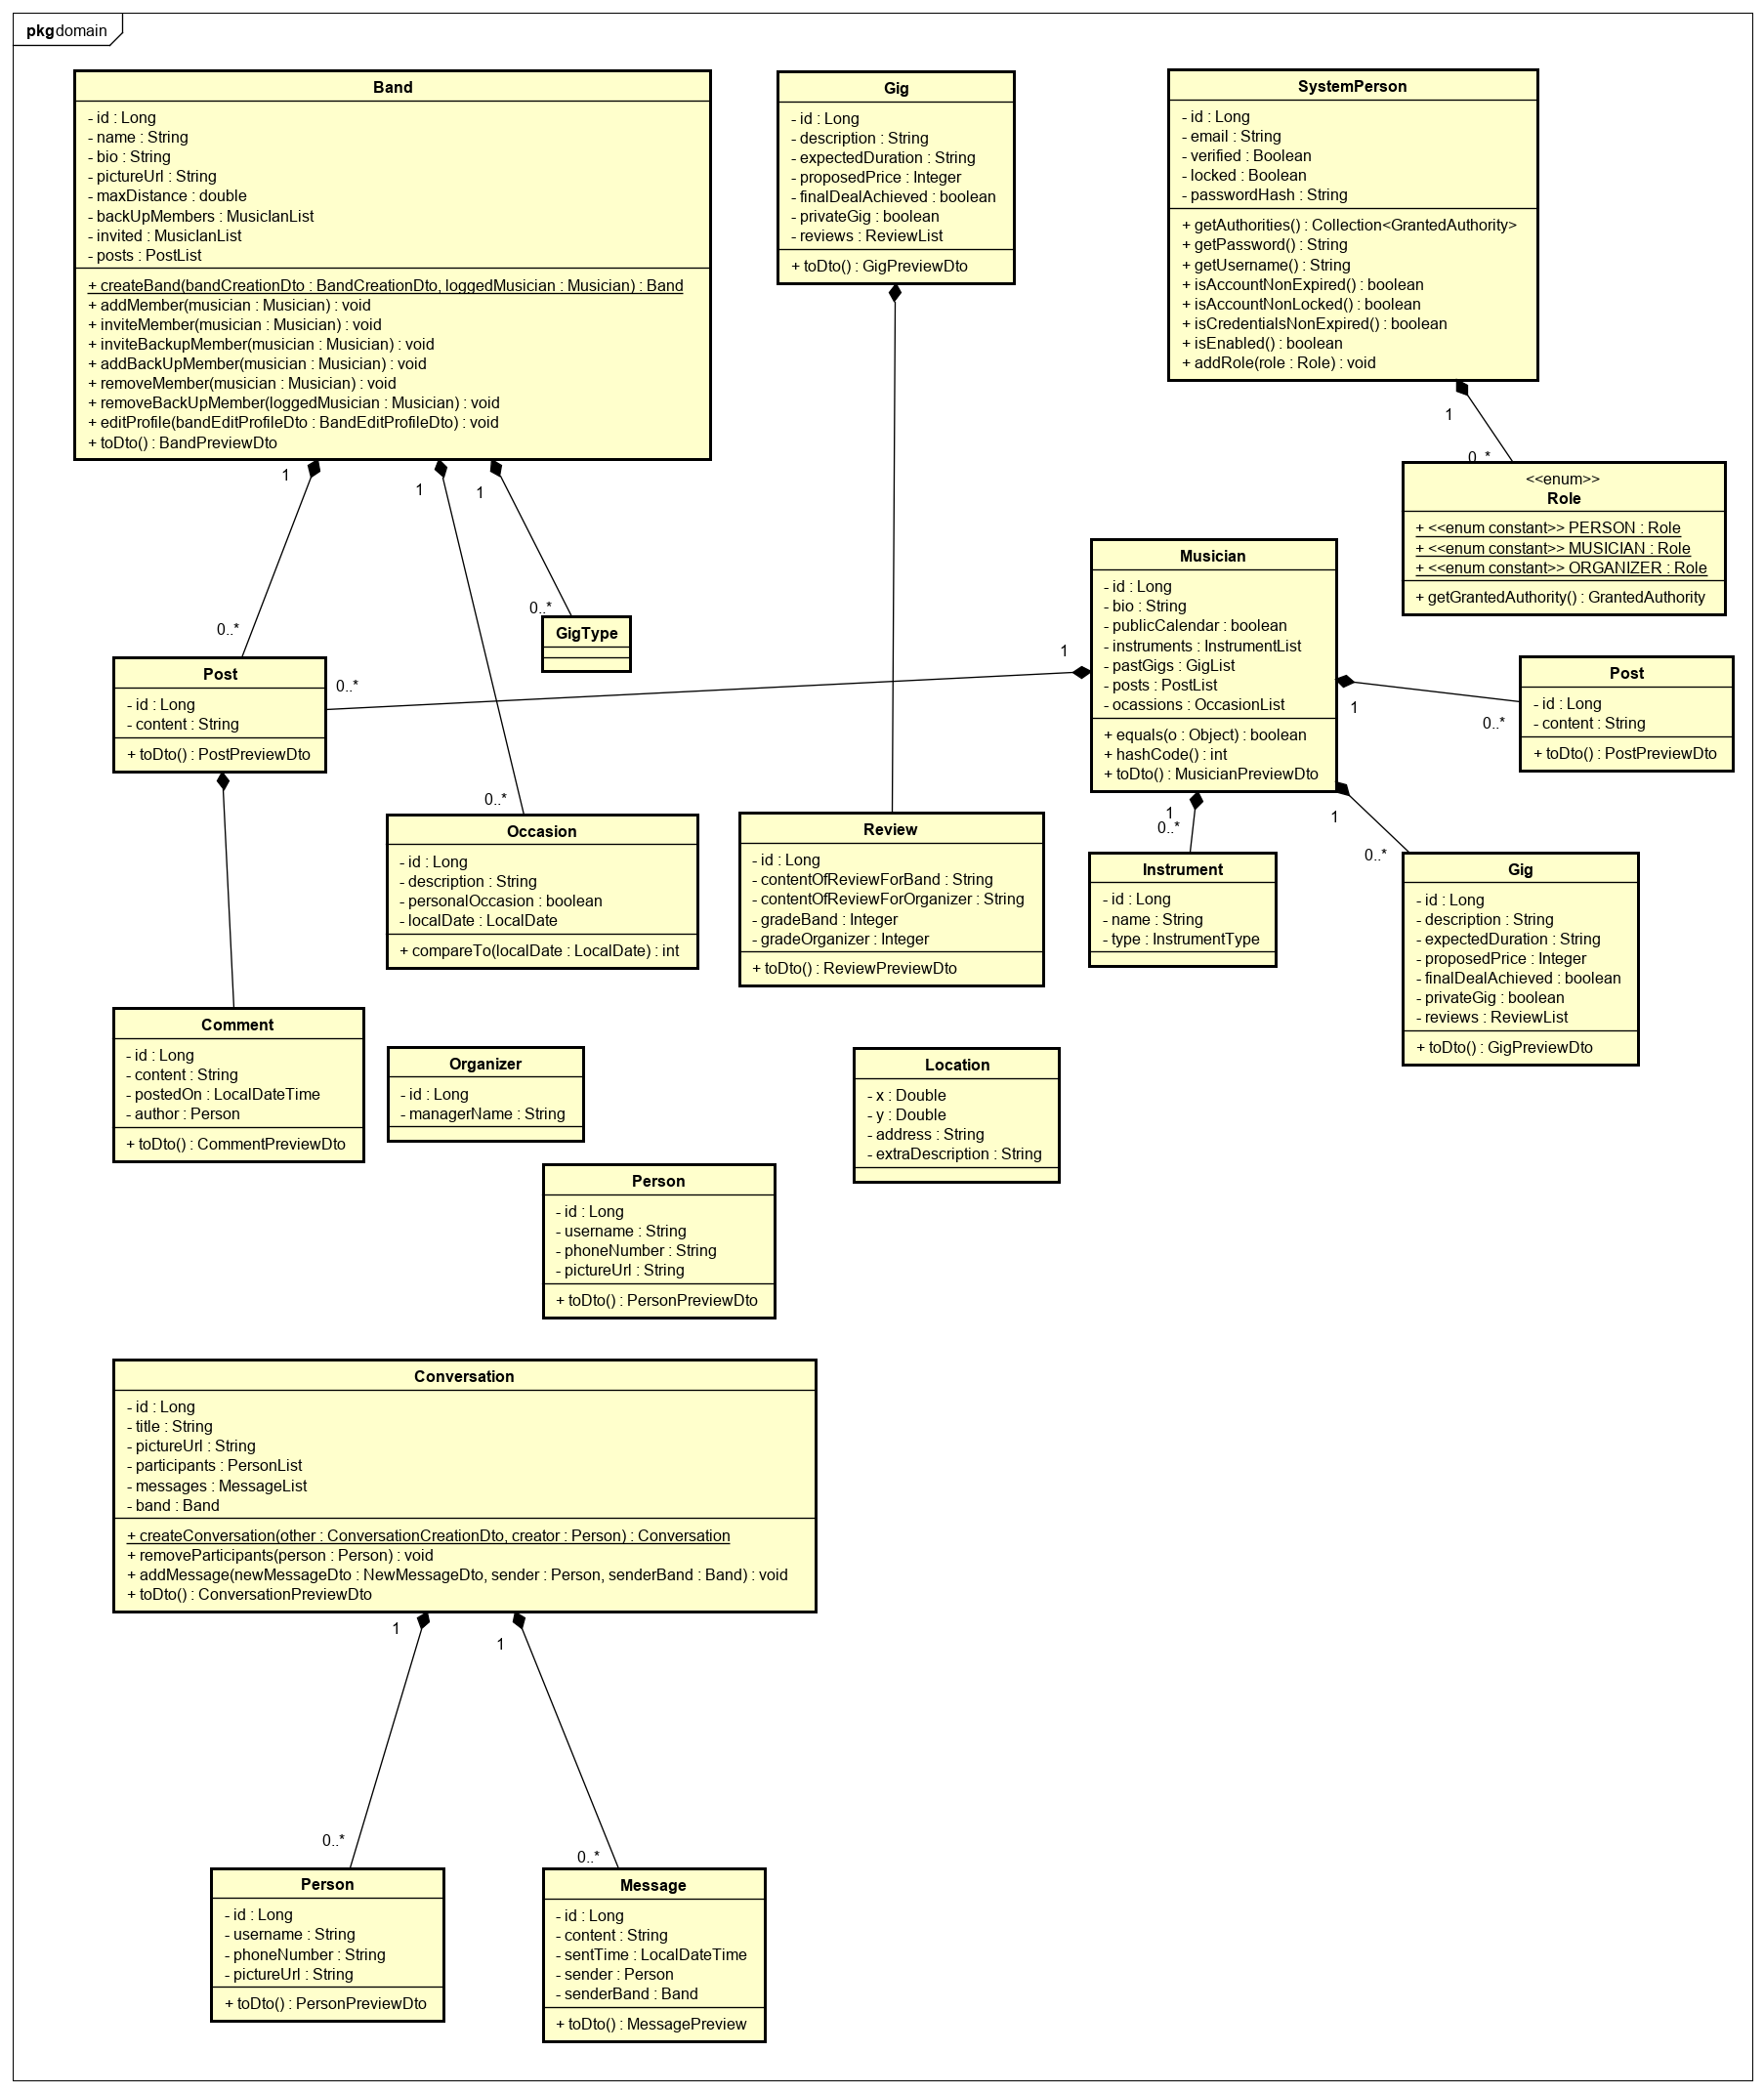
\includegraphics[width=17cm]{slike/domena.PNG}
			\end{center}
			\caption{Dijagram razreda - razredi entiteta}
			\label{fig:domena}
		\end{figure}
		
		\section{Dijagram stanja}
			
			
			\textbf{\textit{dio 2. revizije}}\\
			
			\textit{Potrebno je priložiti dijagram stanja i opisati ga. Dovoljan je jedan dijagram stanja koji prikazuje \textbf{značajan dio funkcionalnosti} sustava. Na primjer, stanja korisničkog sučelja i tijek korištenja neke ključne funkcionalnosti jesu značajan dio sustava, a registracija i prijava nisu. }
			
			
			\eject 
		
		\section{Dijagram aktivnosti}
			
			\textbf{\textit{dio 2. revizije}}\\
			
			 \textit{Potrebno je priložiti dijagram aktivnosti s pripadajućim opisom. Dijagram aktivnosti treba prikazivati značajan dio sustava.}
			
			\eject
		\section{Dijagram komponenti}
		
			\textbf{\textit{dio 2. revizije}}\\
		
			 \textit{Potrebno je priložiti dijagram komponenti s pripadajućim opisom. Dijagram komponenti treba prikazivati strukturu cijele aplikacije.}